\documentclass[fleqn,10pt]{wlscirep}
\usepackage[T1]{fontenc}
\usepackage[utf8]{inputenc}
\usepackage{mathptmx}
\usepackage{booktabs,dcolumn}
\usepackage{color, colortbl}
\usepackage{graphicx}
\usepackage{caption}
\DeclareCaptionLabelFormat{nospace}{#1#2}
\captionsetup[table]{labelfont=bf, name=Table S,labelformat=nospace,labelsep=period}
\captionsetup[figure]{labelfont=bf, name=Figure S,labelformat=nospace,labelsep=period}


\title{ Discovery of Diagnostic and Prognostic long non-coding RNA Biomarkers in Patients with Colorectal Cancer Using Machine Learning Algorithms.}

\author[1]{Zhuha Zhou}
\author[1]{Ximei Ma}
\author[2]{QiuQiang Zhang}
\author[3]{Zhuxian Zhou}

\author[4*]{Ye Feng}
\author[1*]{Guanyu Wang}
\affil[1] {Department of General Surgery, Sir Run Run Shaw Hospital, School of Medicine, Zhejiang University, East Qingchun Road 3, 310016, Hangzhou, Zhejiang, China.}
\affil[2] {Division of Hepatobiliary and Pancreatic Surgery, Second Affiliated Hospital, School of Medicine, Zhejiang University, Jiefang Road 88, 310009, Hangzhou, China. }
\affil[3] {Center for Bionanoengineering and Key Laboratory of Biomass Chemical Engineering of Ministry of Education, College of Chemical and Biological Engineering, Zhejiang University, Zheda Road 38, 310027 Hangzhou, China.}
\affil[4] {Institute of Translational Medicine, School of Medicine, Zhejiang University, East Qingchun Road 3, 310016, Hangzhou, Zhejiang, China.}
\affil[*] {Correspondence and requests for materials should be addressed to (email: wangguanyu@zju.edu.cn)}


\begin{document}
\flushbottom
\maketitle
\begin{table}[!htp]
  \centering
  \caption{Statistical baseline information of clinical features in the training and testing group. }
    \begin{tabular}{llll}
	\toprule[2pt]
          & \multicolumn{2}{c}{\textbf{Group}} &  \\
    \cline{2-3}
    \textbf{Item} & \textbf{Training (n=300)} & \textbf{Testing (n=128)  } & \textbf{p-value} \\
    \midrule[1pt]
    \multicolumn{1}{p{11.3em}}{\textbf{Overall survival (days)}} & 880 ($\pm$752) & 915 ($\pm$864) & 0.689 \\
    \specialrule{0em}{.3em}{.3em}
    \textbf{Age (years)} & 66.1 ($\pm$13.3) & 68.1 ($\pm$12.3) & 0.120 \\
    \specialrule{0em}{.3em}{.3em}
    \textbf{Preoperative CEA (ng/ml)} & 33.6 ($\pm$197) & 50.4 ($\pm$218) & 0.555 \\
     \specialrule{0em}{.3em}{.3em}
    \textbf{Status} &       &       & 1.000 \\
    \hspace{8pt} censored & 234 (78.0\%) & 100 (78.1\%) &  \\
    \hspace{8pt} dead  & 66 (22.0\%) & 28 (21.9\%) &  \\
    \specialrule{0em}{.3em}{.3em}
    \textbf{Gender} &       &       & 0.449 \\
   \hspace{8pt} male  & 156 (52.0\%) & 72 (56.2\%) &  \\
   \hspace{8pt} female & 144 (48.0\%) & 56 (43.8\%) &  \\
    \specialrule{0em}{.3em}{.3em}
    \textbf{Stage} &       &       & 0.988 \\
   \hspace{8pt} i     & 51 (17.0\%) & 22 (17.2\%) &  \\
  \hspace{8pt}  ii    & 117 (39.0\%) & 51 (39.8\%) &  \\
   \hspace{8pt} iii   & 90 (30.0\%) & 36 (28.1\%) &  \\
   \hspace{8pt} iv    & 42 (14.0\%) & 19 (14.8\%) &  \\
      \specialrule{0em}{.3em}{.3em}
    \textbf{Lymphatic invasion} &       &       & 0.909 \\
    \hspace{8pt} no    & 167 (55.7\%) & 69 (53.9\%) &  \\
    \hspace{8pt} yes   & 106 (35.3\%) & 45 (35.2\%) &  \\
   \hspace{8pt}  missing & 27 (9.0\%) & 14 (10.9\%) &  \\
        \specialrule{0em}{.3em}{.3em}
    \textbf{Perineural invasion} &       &       & 0.513 \\
   \hspace{8pt} no    & 98 (32.7\%) & 31 (24.2\%) &  \\
   \hspace{8pt} yes   & 35 (11.7\%) & 8 (6.2\%) &  \\
   \hspace{8pt} missing & 167 (55.7\%) & 89 (69.5\%) &  \\
      \specialrule{0em}{.3em}{.3em}
    \textbf{Venous invasion} &       &       &  \\
   \hspace{8pt} no    & 201 (67.0\%) & 82 (64.1\%) & 0.685 \\
   \hspace{8pt}  yes   & 61 (20.3\%) & 28 (21.9\%) &  \\
   \hspace{8pt}  missing & 38 (12.7\%) & 18 (14.1\%) &  \\
	\bottomrule[2pt]
    \end{tabular}%
  \label{TableS1}%
\end{table}%

\begin{table}[!htbp]
  \centering
    \extrarowheight=\aboverulesep
    \addtolength{\extrarowheight}{\belowrulesep}
    \aboverulesep=0pt
    \belowrulesep=0pt
  \caption{Statistical information of lncRNA features in patient's group.}
    \begin{tabular}{llll}
	\toprule[2pt]
          & \multicolumn{2}{c}{\textbf{Survival Status}} &  \\
          \cline{2-3}
    \textbf{Item} & \multicolumn{1}{p{9.65em}}{\textbf{Censored (n=334)}} & \multicolumn{1}{p{7.7em}}{\textbf{Dead (n=94)}} & \multicolumn{1}{p{4.05em}}{\textbf{P-value}} \\
       \specialrule{0em}{.3em}{.3em}
   \midrule[1pt]
   \textbf{Overall survival (days)} & 940 ($\pm$802) & 717 ($\pm$703) & 0.009 \\
         \specialrule{0em}{.3em}{.3em}
    \textbf{Relative Risk Score} & 1.43 ($\pm$1.98) & 4.92 ($\pm$5.88) & <0.001 \\
          \specialrule{0em}{.3em}{.3em}
    \textbf{Risk Group} &       &       &  \\
   \hspace{8pt} high  & 141 (42.2\%) & 73 (77.7\%) & <0.001 \\
    \hspace{8pt} low   & 193 (57.8\%) & 21 (22.3\%) &  \\
           \specialrule{0em}{.3em}{.3em}
    \textbf{Group} &       &       & 1.000 \\
  \hspace{8pt} Testing & 100 (29.9\%) & 28 (29.8\%) &  \\
  \hspace{8pt} Training & 234 (70.1\%) & 66 (70.2\%) &  \\
          \specialrule{0em}{.3em}{.3em}
    \textbf{LncRNA Expression} &       &       &  \\
          \specialrule{0em}{.3em}{.3em}
   \hspace{8pt} RP11-440D17.3 & -0.203 ($\pm$2.29) & 0.158 ($\pm$2.39) & 0.194 \\
         \specialrule{0em}{.03em}{.03em}
  \hspace{8pt} EIF3J-AS1 & 0.876 ($\pm$0.564) & 1.04 ($\pm$0.567) & 0.012 \\
        \specialrule{0em}{.03em}{.03em}
   \hspace{8pt} TNRC6C-AS1 & 0.432 ($\pm$0.906) & 0.705 ($\pm$0.917) & 0.012 \\
        \specialrule{0em}{.03em}{.03em}
   \hspace{8pt} MIR210HG & 1.26 ($\pm$1.24) & 1.63 ($\pm$1.23) & 0.011 \\
        \specialrule{0em}{.03em}{.03em}
   \hspace{8pt} AC113189.5 & 1.35 ($\pm$0.727) & 1.66 ($\pm$0.913) & 0.003 \\
        \specialrule{0em}{.03em}{.03em}
   \hspace{8pt} LINC00261 & 1.48 ($\pm$2.18) & 0.803 ($\pm$2.07) & 0.006 \\
       \specialrule{0em}{.03em}{.03em}
   \hspace{8pt} CTB-25B13.12 & 2.15 ($\pm$0.708) & 2.45 ($\pm$0.639) & <0.001 \\
       \specialrule{0em}{.03em}{.03em}
  \hspace{8pt}  AC114730.3 & 1.20 ($\pm$1.43) & 0.788 ($\pm$1.89) & 0.053 \\
	\bottomrule[1.5pt]
    \end{tabular}%
  \label{TableS2}%
\end{table}%

\begin{figure}[!h]
\centering
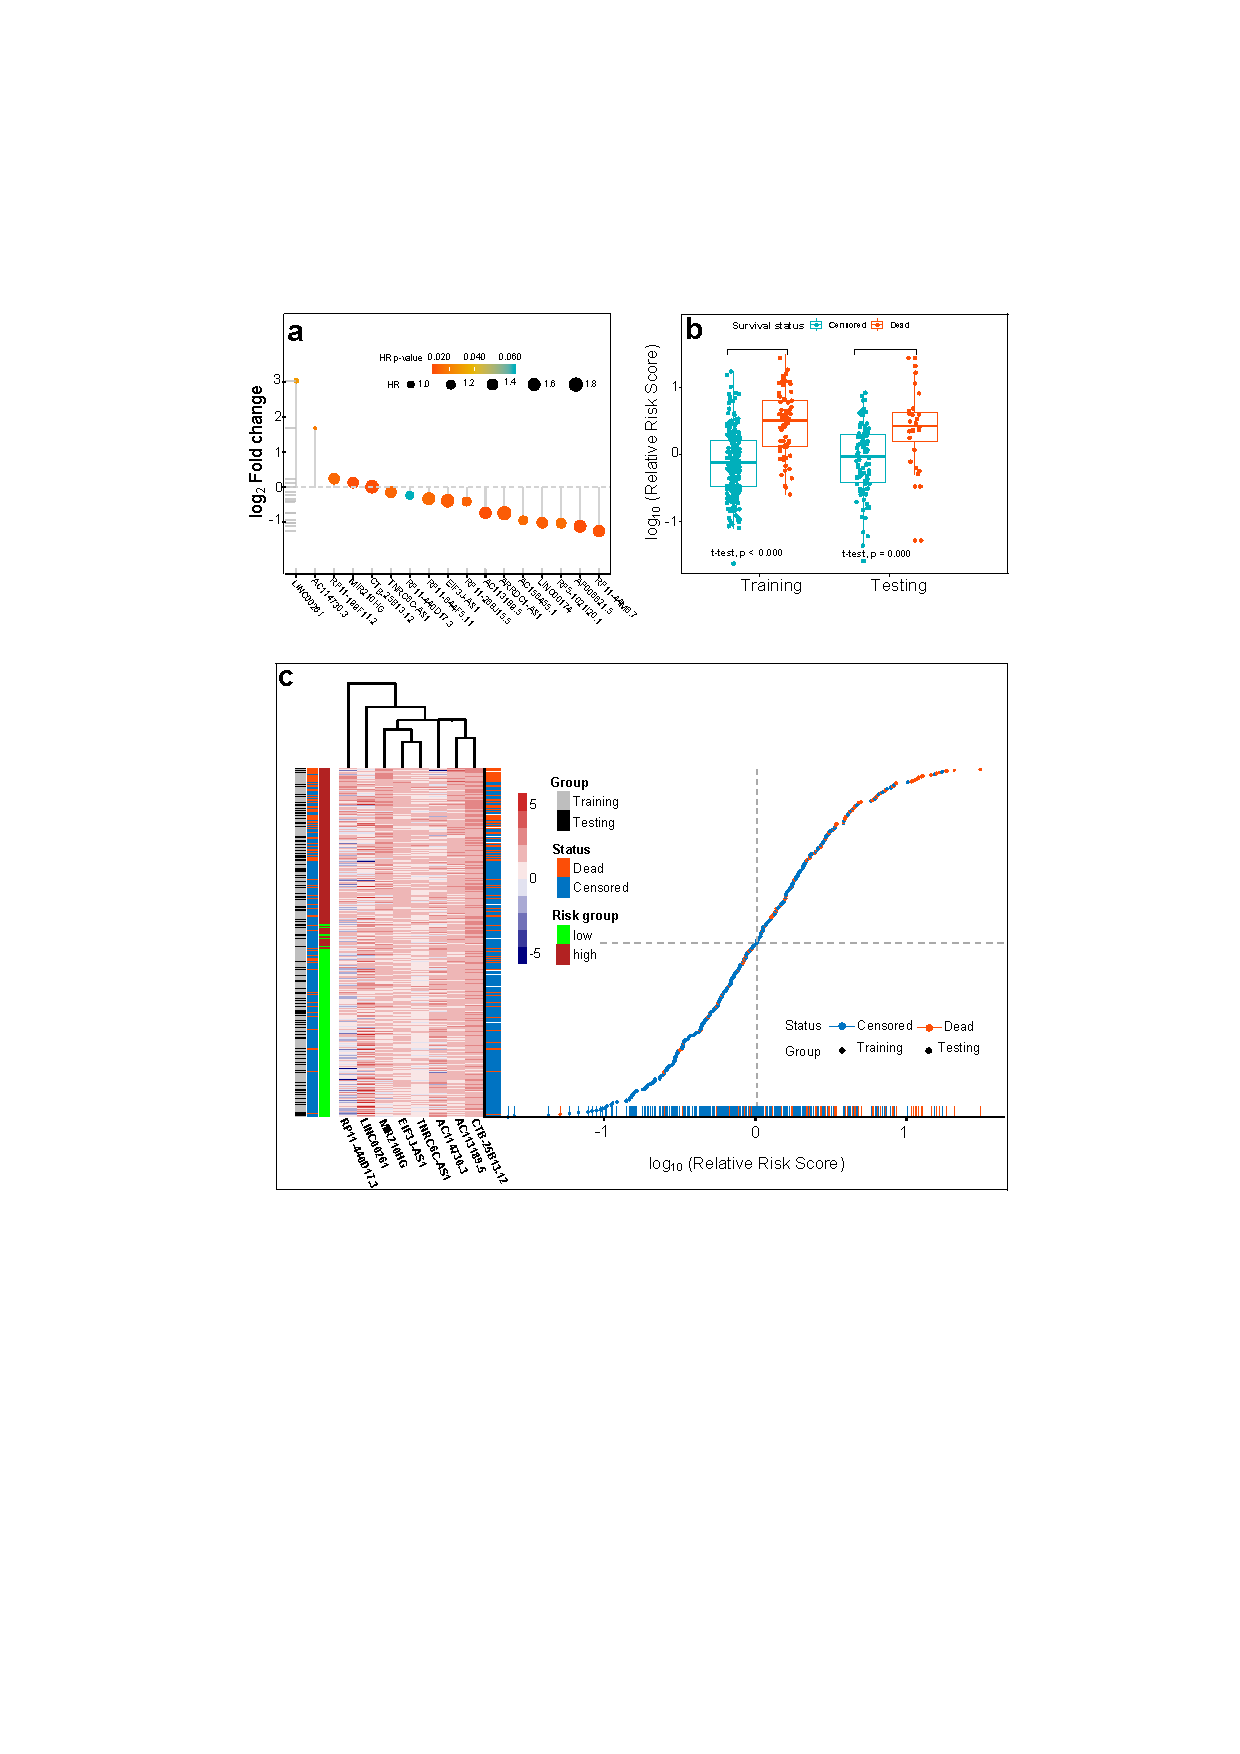
\includegraphics[width=1\textwidth]{Figure-S1-Guanyu}       
\caption{(a) The features of the 17 candidate lncRNAs : HR was depicted as the size of dots with corresponding  color annotated p-value, and $\log_{2}$ FC as the y-axis. Most of the downregulated lncRNAs associated with increased HR, while LINC00261, a putative negative regulator of cell growth through promoting differentiation and apoptosis was significantly upregulated with decreased HR. (b) Boxplot of $\log_{10}(Relative Risk Score)$ in groups: $\log_{10}(Relative Risk Score)$ were significant higher in the patient suffering from death of CRC in both groups. (c) The patients' relative risk score distribution and lncRNA expression heatmap: The patients were evenly partitioned in training and testing group as the grey and black legend bar shown. Relative Risk Score stratified patients into high and low risk group shown as dark-red and green bar. The death experienced and high risked patients mainly clustered in the upright region on the graph.}
\label{FigS1}
\end{figure}


\begin{figure}[!h]
\centering
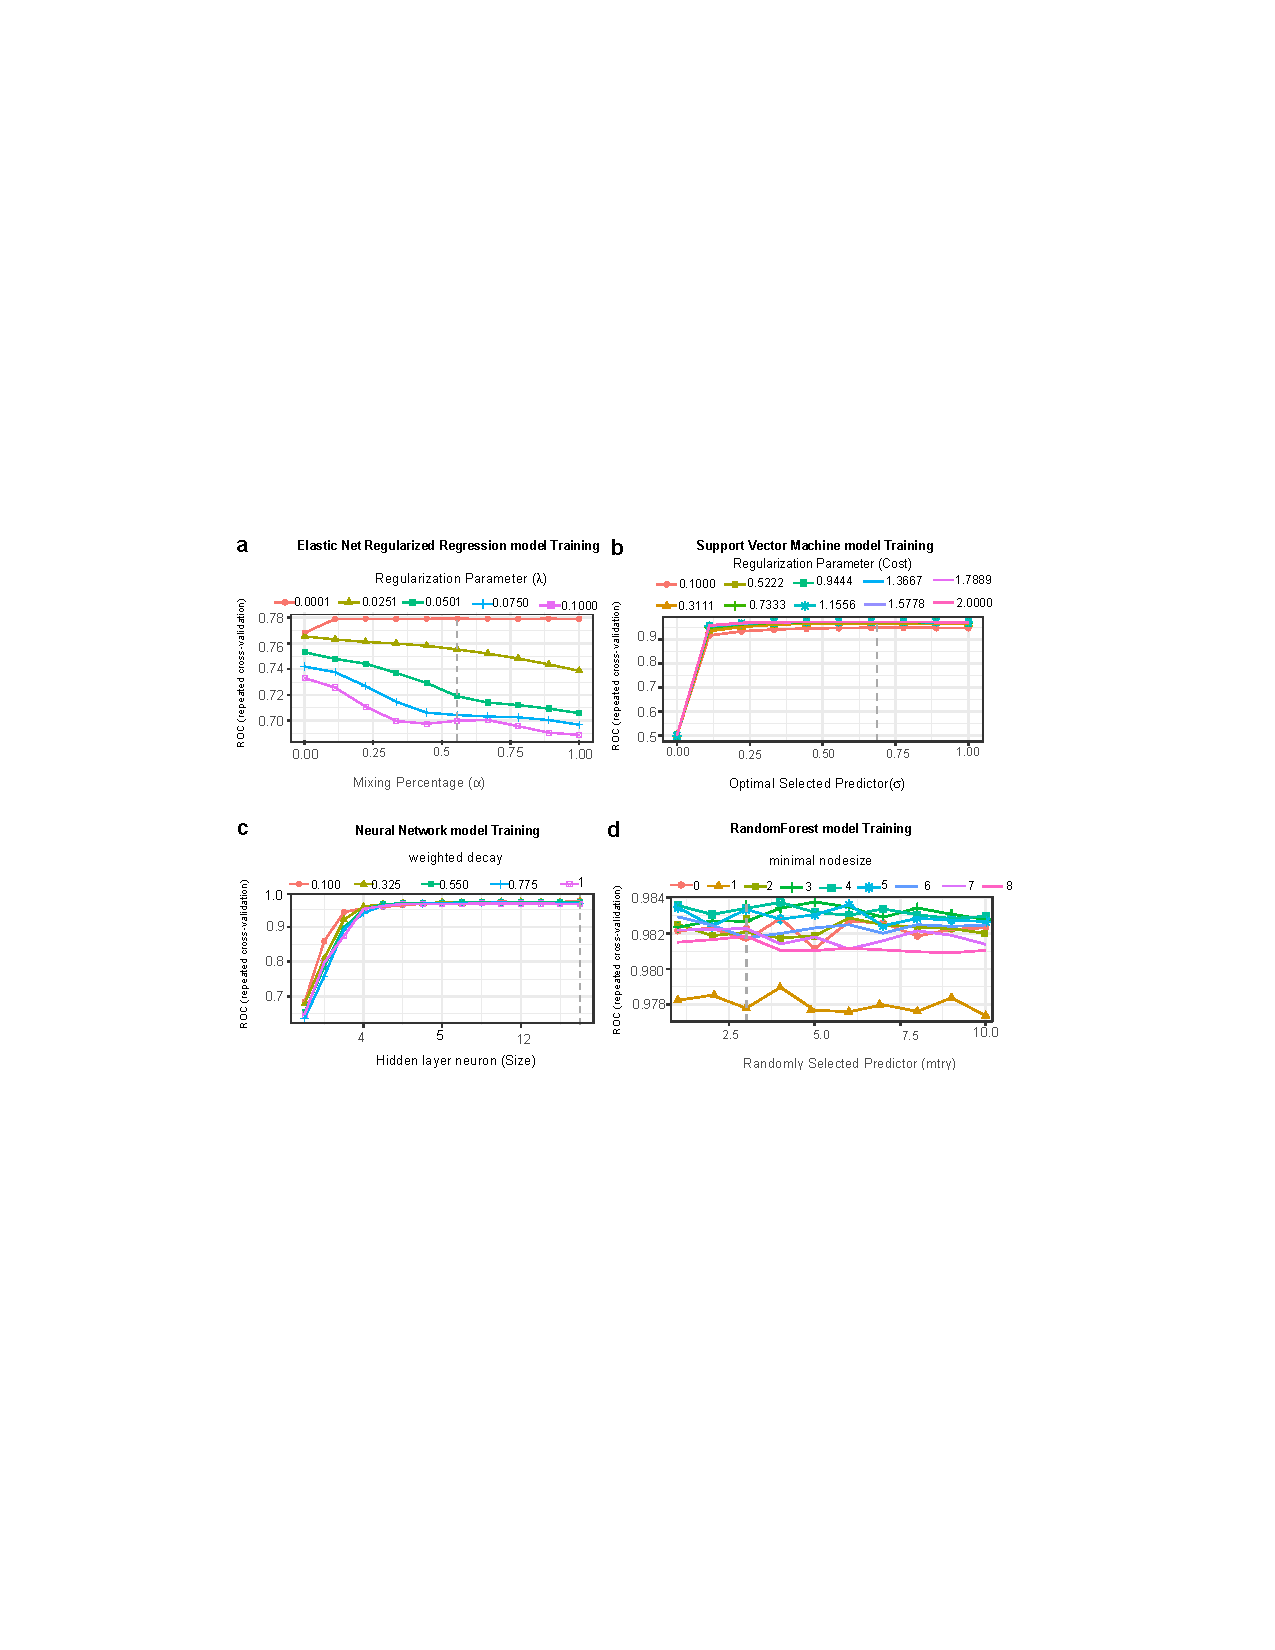
\includegraphics[width=1\textwidth]{Figure-S2-Guanyu}       
\caption{Repeated cross-validated ROC and optimal tuning hyperparameter in each classification model: Each dashed vertical line indicating where the optimal point located. (a) Elastic net regularized regression model ($\alpha = 0.556$, $\lambda = 1\times10^{-4}$). (b) Support vector machine model ($Cost = 0.944$, $\sigma = 0.667$), (c) Neural network model ($Size = 15$, $decay = 0.100$), (d) Random forest model ($mtry = 3$, $minimal$ $nodesize = 5$)}
\label{FigS2}
\end{figure}

\end{document} 